\chapter{Modelli a singola coda}
Un modello a cosa è costituito dalla rappresentazione di un sistema di congestione in cui utenti che provengono da una popolazione si mettono in coda per ottenere il servizio richiesto da un insieme di risorse o serventi. Una coda è una linea di attesa per un servizio. L'insieme formato da cosa e serventi è detto \textbf{centro di servizio}. 

\begin{figure}[H]
	\centering
    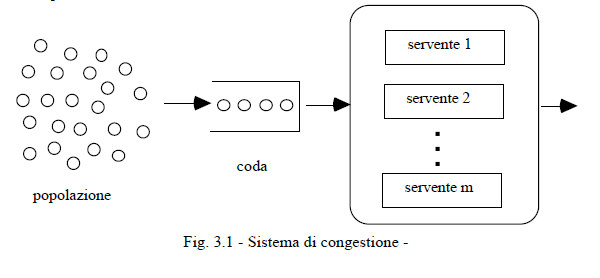
\includegraphics[width=15cm, keepaspectratio]{img/modello_coda.png}
	\caption{Sistema di congestione.}\label{fig:modello_coda}
\end{figure}
Un sistema a coda è costituito da alcune grandezze che sono:
\begin{itemize}
    \item $\Delta$ tempo di interarrivo;
    \item w numero di utenti in cosa e $t_w$ tempi di attesa in coda, tempo che intercorre fra l'arrivo di un utente e l'istante in cui entra in servizio;
    \item s numero di utenti in coda e $t_s$ tempo di servizio, tempo fra inizio e completamento del servizio;
    \item q numero di utenti nel sistema e $t_q$ tempo di risposta, tempo fra arrivo e partenza dal sistema dello stesso utente.
\end{itemize}
Per definizione $q= w+s$ e le variabili di tempi sono legati dalla seguente relazione $t_q = t_w + t_s$.

Fra queste tipicamente alcune sono parametri del sistema, quali $t_s$ e $\Delta$ mentre le altre sono oggetto di analisi e di valutazione.
\paragraph{Processo di arrivo}
Assumiamo che il tempi di interarrivo $ \Delta$ siano variabili casuali statisticamente indipendenti con la stessa distribuzione di probabilità.
\paragraph{Domanda di servizio, tasso di servizio e tempo di servizio}
La quantità di servizio richiesta da un utente ad un centro di servizio è detta
domanda di servizio ed è espressa in unità di tempo. La velocità o tasso di servizio di un servente è una caratteristica del servente, ovvero della risorsa, ed è espressa in unità di servizio per unità di tempo. Il tempo di servizio è la il rapporto fra la domanda di servizio e la velocità di servizio espresso in unità di tempo.
\paragraph{Disciplina di servizio}
Una \textbf{disciplina di servizio} è un algoritmo di ordinamento degli utenti in coda in base al quale viene selezionato l'utente da servire, ovvero l’ordine con cui estrarre gli utenti dalla coda. Alcuni esempi sono FIFO che serve gli utenti in ordine di arrivo  e LIFO che serve gli utenti in ordine inverso al tempo di
arrivo. La disciplina di servizio RAND determina l’utente da estrarre dalla coda e servire
in modo casuale, secondo la distribuzione unforme discreta. Le \textbf{discipline a priorità} determinano l’ordine di servizio degli utenti sulla base di priorità assegnate ad esse. La disciplina round robin è un esempio di disciplina che dipende dalla quantità di servizio già assegnato. Tale algoritmo assegna il servente ciclicamente agli utenti per un intervallo massimo di tempo detto quanto.

\subsection{Notazione di Kendall} Per descrivere e definire i modelli a coda singola Kendall
ha introdotto la seguente notazione:
\[ A/B/c/n/p/Z\]
dove i simboli denotano:
\begin{itemize}
    \item A : distribuzione del tempo di interarrivo;
    \item B : distribuzione del tempo di servizio $t_s$;
    \item c : numero di serventi m;
    \item n : dimensione della coda ovvero la capacità del centro, q;
    \item p : dimensione della popolazione;
    \item  Z : disciplina di servizio.
\end{itemize}
 Tale notazione si semplifica in A/B/c quando coda e popolazione sono illimitate e
la disciplina di servizio è FIFO, ovvero se $n=p=\infty$ e Z=FIFO. D denota la distribuzione deterministica o costante, M la distribuzione esponenziale negativa,$H_h$ l’iperesponenziale ad h stadi,$E_k$ l’Erlangiana a k stadi e G la generale.
Il comportamento del sistema nel tempo può essere analizzato in un tempo finito.
In tal caso si parla di \textbf{analisi transiente}. Quando il sistema raggiunge le condizioni di
equilibrio in un tempo che tende ad infinito, ovvero se il sistema è stabile si effettua
\textbf{l’analisi stazionaria.} Tale analisi porta alla valutazione degli indici di prestazione del sistema di code, in particolare di:
\begin{itemize}
    \item numero di utenti nel sistema q;
    \item numero di utenti in coda w;
    \item tempo di risposta $t_q$;
    \item tempo di attesa $t_w$;
    \item utilizzazione U;
    \item throughput X.
\end{itemize}
Le prime quattro sono variabili casuali di cui si valuta la distribuzione di probabilità,
e/o i momenti. Possiamo scrivere immediatamente le seguenti
relazioni fra i valori medi:

\begin{align}
    & E[q] = E[w] + E[s]\\
    & E[t_q] = E[t_w] + E[t_s]
\end{align}

Una relazione fondamentale nella teoria delle code è rappresentato dal \textbf{teorema di
Little} il quale stabilisce che il numero medio di utenti in un sistema è uguale al
prodotto fra il throughput e il tempo medio di risposta, ovvero:

\begin{align}
   & E[q] = X E[t_q] \\
   & E[w] = X E[t_w]
\end{align}

\subsection{Modelli basilari di code: i sistemi M/M/1 ed M/M/m}
M/M/1 costituisce la base per la definizione di modelli più
complessi a struttura reticolare e per lo sviluppo gerarchico di modelli a diversi livelli
di astrazione. Nella notazione di Kendall il sistema di code M/M/1 denota un sistema aperto
formato da un singolo centro di servizio con:
\begin{itemize}
    \item distribuzione del tempo di interarrivo esponenziale, di parametro $\lambda$,
    \item tempo di servizio degli utenti indipendente e con identica distribuzione
esponenziale di parametro $\mu$,
    \item singolo servente.
\end{itemize}
La disciplina di servizio è FIFO e sia la memoria che la popolazione sono infinite.
\begin{figure}[H]
	\centering
    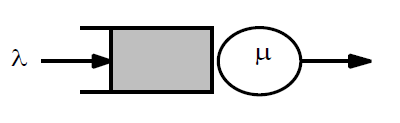
\includegraphics[width=13cm, keepaspectratio]{img/sistema_mm1.png}
	\caption{Sistema M/M/1.}\label{fig:mm1}
\end{figure}

Per le ipotesi di esponenzialità dei tempi di interarrivo e di servizio, gli unici eventi possibili che si osservano in un intervallo di tempo $d_t$ quando nel sistema vi sono k utenti sono i seguenti:
\begin{enumerate}
    \item nessun arrivo e nessun completamento di servizio (permanenza nello stato k);
    \item un arrivo e nessun completamento di servizio (transizione dallo stato k allo stato k+1
con probabilità $\lambda dt$);
    \item nessun arrivo e un completamento di servizio (transizione dallo stato k allo stato k-1
con probabilità $\mu dt$);
    \item uno o più arrivi e uno o più completamenti di servizio (transizione con probabilità
trascurabile rispetto alle altre transizioni per l’ipotesi di esponenzialità).
\end{enumerate}

\subsection{Analisi stazionaria}
Definiamo l’intensità di traffico del sistema come rapporto fra tempo medio di servizio e tempo medio di interarrivo, denotato da $\rho = \lambda / \mu$. La condizione di
stazionarietà del sistema M/M/1 richiede che $\rho <1$, ovvero che il tasso di arrivo al
sistema sia minore del tasso di servizio, $\lambda < \mu$. La distribuzione di probabilità di stato in
equilibrio  si ricava :
\begin{align}
    & \pi_0 = 1- \rho \\
    &\pi_k = \rho^k \pi_0 = \rho (1-\rho) & k>0
\end{align}
la distribuzione di probabilità del numero di utenti nel sistema in condizioni stazionarie è geometrica a ragione $\rho$. \\
Il numero medio di utenti nel sistema, che denotiamo con N=E[q], si può immediatamente ricavare come:
\begin{align}
    N = \frac{\rho }{1-\rho} 
\end{align}
e la varianza del numero di utenti, denotata da Var[q], è
\begin{align}
    Var[q] = \frac{\rho}{(1-\rho)^2}
\end{align}
Per la relazione (5.1) ricaviamo immediatamente il numero medio di utenti in coda,
denotato da W=E[w], poiché $E[s] =\rho$ ed E[q]=N:
\begin{align}
    W = N-\rho = \frac{\rho^2 }{1-\rho}
\end{align}

Il tempo medio di risposta, denotato da R=E[tq], si ricava dal teorema di Little  che per il sistema M/M/1 assume la forma $N= \lambda R$:
\begin{align}
    R = \frac{\frac{1}{\mu}}{1-\rho}
\end{align}

Infine il tempo medio di attesa in coda,$T_w=E[t_w]$ si ottiene o dal teorema di Little come $W = \lambda T_w$ o dalla relazione (3.4) ovvero $R = T_w +T_s$, dove $T_s = \frac{1}{\mu}$ denota il tempo medio di servizio, da cui si ricava
\begin{align}
    T_w = \frac{\frac{\rho}{\mu}}{1-\rho}
\end{align}

L’utilizzazione è esprimibile per il sistema M/M/1 come:
\begin{align}
    U = 1 -\pi_0 = \rho
\end{align}

Dalla distribuzione di probabilità (5.6) possiamo calcolare la probabilità con cui si
osservano almeno k utenti nel sistema in condizioni di equilibrio:
\begin{align}
    & Prob \{ \textrm{numero di utenti nel sistema $\geq$ k}\}= \sum_{i\geq k}^{} \pi_i= (1-\rho) \sum_{i\geq k}^{} \rho_i =\rho^k
\end{align}

\subsection{Sistema M/M/$\infty$ : serventi infiniti}
Un modello M/M/$\infty$ permette di rappresentare un sistema nel quale ad ogni
arrivo vi è sempre un servente libero.In un sistema di questo tipo non si forma quindi
mai coda, poiché ogni utente riceve immediatamente servizio dall’istante in cui arriva
al sistema. Il processo stocastico {q(t) | t>0} associato al sistema $M/M/\infty$ è un processo di
nascita e morte con tassi di nascita $\lambda_k=\lambda, k\geq0, $e con tassi di morte $\mu_k= k \mu, k\geq1$. La condizione di stazionarietà è certamente sempre soddisfatta quindi il
sistema è sempre stabile. esiste la distribuzione stazionaria del numero di utenti nel
sistema, che coincide con il numero di serventi occupati da cui si ricava:
\begin{align}
    & \pi_k = \frac{\rho^k}{k!} e^{-\rho} & k\geq 0
\end{align}
dove $\rho = \lambda/\mu$.
Si ricava immediatamente il numero medio di utenti nel sistema 
\begin{align}
    N = \rho
\end{align}
Dato che nel sistema $M/M/\infty $ gli utenti non sperimentano mai coda, il tempo medio
di risposta coincide con il tempo medio di servizio:
\begin{align}
    R = T_s = \frac{1}{\mu}
\end{align}

\subsection{Sistema M/M/m: serventi multipli}
Il sistema aperto M/M/m è caratterizzato da un processo di arrivo Poissoniano di $\lambda$
parametro, distribuzione del tempo di servizio esponenziale di parametro $\mu$ e un
numero di serventi m>0. Come in M/M/1  il tasso medio di servizio dipende dallo stato k secondo la seguente funzione $\mu(k) = k \mu$ ,$0\leq k\leq m, e \mu(k) = m \mu, k>m$.  Definiamo l’intensità di traffico come $\rho =\lambda/ m\mu$. In questo caso esiste la distribuzione stazionaria del numero di utenti nel sistema :
\begin{align}
    & \pi_k = \frac{(m\rho)^k}{k!}\pi_0 & 0\leq k \leq m \\
    &\pi_k = \frac{m^m \rho^k}{m!}\pi_0 & k>m \\
    &\pi_0 = \left [  \sum_{k=0}^{m-1} \frac{(m\rho)^k}{k!} +  \frac{(m\rho)^m}{m!}\cdot \frac{1}{1-\rho} \right ]^{-1}
\end{align}
Il numero medio di serventi occupati E[s] è dato da
\begin{align}
    & E[s] = \sum_{k=0}^{m-1} k \pi_k + \frac{m\pi_m}{1-\rho} = m\rho = \frac{\lambda}{\mu}
\end{align}
dove $\rho$ rappresenta l’utilizzazione di ogni singolo servente.
Il numero medio di utenti nel sistema è dato da
\begin{align}
    & N = m \rho + \pi_m \frac{\rho}{(1-\rho)^2} \\
    & W = \pi_m \frac{\rho}{(1-\rho)^2}
\end{align}
Il tempo medio di risposta si ottiene applicando il teorema di Little $N=\lambda R$ ottenendo:
\begin{align}
    R = \frac{1}{\mu} + \frac{\pi_m}{(m\mu(1-\rho)^2)}
\end{align}

Similmente, otteniamo il tempo medio di attesa:
\begin{align}
    T_W = \frac{\pi_m}{m\mu ( 1-\rho)^2}
\end{align}
La probabilità che un utente in arrivo trovi tutti i serventi occupati e quindi
sperimenti coda è data dalla formula di Erlang-C:
\begin{align}
    Prob\{\textrm{coda}\} = \sum_{k=m}^{\infty}\pi_k = \pi_0 \frac{(m\rho)^m}{!m} \cdot \frac{1}{1-\rho}
\end{align}
Questa formula, è stata applicata per lo studio di sistemi di traffico telefonico per valutare la probabilità che una chiamata (un utente) trovi tutti i canali di comunicazione (i serventi) occupati.
\\
Vedere esercizio \ref{es:m/m/m}.

\subsection{Sistema M/M/1/K : memoria finita}
Consideriamo il sistema M/M/1 nel quale sono ammessi al più K utenti. Il processo di arrivo è Poissoniano di parametro $\lambda$, ma un utente che arrivando trova il sistema completo, cioè con K utenti già presenti, non viene accettato e viene perso. Il processo stocastico ${q(t) | t>0}$ associato al sistema M/M/1/k è un processo di nascita e morte con spazio degli stati finito $E=\{0,1,\cdots, K\}$ e tassi di nascita $\lambda_k=\lambda$,$ 0 \leq k<K$, e tassi di morte $\mu_k= \mu$, $1\leq k<K-1$ e $\lambda_k=0$ e $\mu_k= 0$ altrove. La condizione di stazionarietà è certamente verificata, poiché il processo è finito e irriducibile e quindi ergodico. La distribuzione stazionaria del numero di utenti nel sistema
definita dalle formule:
\begin{align}
    & \pi_k = \frac{1-\rho}{1 -\rho^{K+1}} \rho & 0\leq k \leq K \\
    & \pi_k = 0 & k>K
\end{align}
Nel caso particolare di K=1 lo spazio è formato da due soli stati e si ricava
\begin{align}
    & \pi_0 = \frac{\mu}{\lambda +\mu}\\
    & \pi_1 = \frac{\lambda}{\lambda + \mu}
\end{align}

\subsection{Sistema M/M/1//M: popolazione finita}
Consideriamo il sistema M/M/1 assumendo che gli utenti provengano da una popolazione finita, di dimensione M>0.